% Shared preamble for the paper. Section files are \input into main.tex and must compile with exactly this.
\documentclass[11pt]{amsart}
\usepackage[utf8]{inputenc}
% T1 encoding omitted: without Latin Modern installed it selects bitmap fonts; the default encoding gives Type 1 Computer Modern.
\usepackage{amsmath,amssymb,amsthm,mathtools}
\usepackage{booktabs,array,longtable}
\usepackage{graphicx}
\usepackage[margin=1.15in]{geometry}
\usepackage[colorlinks=true,linkcolor=black,citecolor=black,urlcolor=black]{hyperref}
\numberwithin{equation}{section}
\newtheorem{theorem}{Theorem}[section]
\newtheorem{lemma}[theorem]{Lemma}
\newtheorem{proposition}[theorem]{Proposition}
\newtheorem{corollary}[theorem]{Corollary}
\theoremstyle{definition}
\newtheorem{definition}[theorem]{Definition}
\newtheorem{hypothesis}[theorem]{Hypothesis}
\newtheorem{observation}[theorem]{Observation}
\theoremstyle{remark}
\newtheorem{remark}[theorem]{Remark}
\newcommand{\R}{\mathbb{R}}
\newcommand{\Z}{\mathbb{Z}}
\newcommand{\N}{\mathbb{N}}
\newcommand{\SU}{\mathrm{SU}}
\newcommand{\U}{\mathrm{U}}
\newcommand{\Tr}{\operatorname{Tr}}
\newcommand{\Cov}{\operatorname{Cov}}
\newcommand{\Var}{\operatorname{Var}}
\newcommand{\cL}{\mathcal{L}}
\newcommand{\cH}{\mathcal{H}}
\newcommand{\cG}{\mathcal{G}}
\newcommand{\E}{\mathbb{E}}
\renewcommand{\P}{\mathbb{P}}
\newcommand{\repo}[1]{\texttt{#1}}
\setlength{\abovecaptionskip}{6pt}

\usepackage{tikz}
\usetikzlibrary{positioning,arrows.meta}
\title[Spectral criteria and conditional infrared estimates]{Spectral criteria and conditional infrared estimates\\ for four-dimensional lattice Yang--Mills theory}
\author{Kirtus Justus}
\address{Theoretical Physicist, Port Coquitlam, British Columbia, Canada}
\date{24 November 2026}
\begin{document}
\begin{abstract}
We prove a spectral criterion for a mass gap, a refinement inequality that tolerates an exceptional set of
coarse fields, and a bound on the return to such a set for $\SU(2)$ Wilson lattice gauge theory in four
dimensions. Two interacting estimates that the refinement inequality needs are not proved; we state them and
report measurements that bear on them. No mass gap is proved.
\end{abstract}
\maketitle
\tableofcontents

\section{Introduction}\label{s:intro}

The problem of Jaffe and Witten~\cite[\S4]{JW} asks, for every compact simple gauge group $G$, for a
non-trivial quantum Yang--Mills theory on $\R^4$ satisfying the Wightman or Osterwalder--Schrader axioms, and
for a mass gap: a number $\Delta>0$ such that the Hamiltonian $H$ has no spectrum in $(0,\Delta)$. This paper
does not solve that problem and does not solve any part of it for the continuum theory. It contains four
proved statements about objects that occur on the way, two named hypotheses that are open, and numerical
measurements. The proved statements are as follows.

\begin{theorem}[Spectral criterion]\label{t:crit}
Let $H\ge0$ be a self-adjoint operator on a Hilbert space $\cH$, let $\tau>0$, and let $D\subset\cH$ have dense
linear span. For $v\in\cH$ and $n\ge0$ put
\[
d_{v,n}=\big\langle v,\,e^{-n\tau H}\big(I-e^{-\tau H}\big)v\big\rangle\ \ge0 .
\]
Let $0<r<1$ and $\Delta=-\tau^{-1}\log r$. The following are equivalent.
\begin{enumerate}
\item $H$ has no spectrum in $(0,\Delta)$.
\item $\limsup_{n\to\infty}d_{v,n}^{1/n}\le r$ for every $v\in D$.
\end{enumerate}
\end{theorem}

No uniformity in $v$ of constants or of the onset of the decay is required in (2); only the rate $r$ is
common. The zero-energy sector, whatever its dimension, contributes nothing to $d_{v,n}$.

\begin{theorem}[Refinement with an exceptional set]\label{t:inh}
Let $H\ge0$ be self-adjoint on a Hilbert space $\mathcal K$, $S_s=e^{-sH}$, and $\lambda=\inf\sigma(H)$. Let
$P$ be an orthogonal projection, $Q=I-P$, and let $B$ be an orthogonal projection with range inside the range
of $Q$; put $G=Q-B$. Let $a>0$, $t>0$, $0<\tau\le t$, $\gamma>0$, $\kappa\ge0$ and $b\in\R$, and suppose
\begin{equation}\label{e:hyp}
\langle f,(I-S_{2a})f\rangle\ge\gamma\|Gf\|^2\ \ (f\in\mathcal K),\qquad
\|BS_\tau B\|\le\kappa,\qquad \|PS_tP\|\le1-b .
\end{equation}
Then the deficit $d=1-\|S_t\|=1-e^{-t\lambda}$ satisfies
\begin{equation}\label{e:inh}
d\ \ge\ \frac{(b-\kappa)_+}{1+2a/(\gamma t)} .
\end{equation}
\end{theorem}

In the application $\mathcal K$ is the space of centred gauge-invariant functions of a time slice of a fine
lattice, $S_s$ is the transfer semigroup normalised by the vacuum, $P$ is the conditional expectation given
the coarse links, $B$ is the part of $Q$ supported on an exceptional set of coarse fields, $a$ is the fine
mesh, and $b$ is a deficit inherited from the coarse lattice. The three inequalities~\eqref{e:hyp} are then:
mixing of fine fluctuations off the exceptional set at rate $\gamma$ per mesh; return to the exceptional set
with weight at most $\kappa$; and a comparison between the fine transfer compressed to coarse functions and
the coarse transfer. Only the second is proved here, for a narrow exceptional set.

\begin{theorem}[Return to a coarse plaquette gate]\label{t:ret}
Consider the Wilson measure with weight $\exp\big(\beta\sum_p\tfrac12\Tr U_p\big)$, $\beta\ge0$, for $G=\SU(2)$
on a periodic lattice with even spatial side $N\ge4$ and $T\ge2$ time slices. Fix a spatial
plaquette of side two (a coarse plaquette) and $0\le\theta\le\pi$, and let $A_\theta$ be the event, for a time
slice, that the holonomy around it lies within round distance $\theta$ of $-I$. Let $x$ and $y$ be the
configurations of two distinct time slices. Then, for every square-integrable function $g$ of a slice,
\begin{equation}\label{e:ret}
\big|\E\big[\mathbf 1_{A_\theta}(x)g(x)\,\mathbf 1_{A_\theta}(y)g(y)\big]\big|\ \le\ p_{6\beta}(\theta)\,
\E\big[\mathbf 1_{A_\theta}(x)g(x)^2\big],
\qquad
p_k(\theta)=\frac{\int_0^\theta\sin^2\!r\,e^{k(\cos r-1)}\,dr}{\int_0^\pi\sin^2\!r\,e^{k(\cos r-1)}\,dr},
\end{equation}
and $p_k(\theta)\le\min\{1,\ \tfrac{\pi^2\sqrt e}{4}(1+k)^{3/2}\theta^3\}$.
\end{theorem}

The bound is uniform in the spatial volume, in the time separation and in the rest of the field. It is a
statement about the lattice with periodic time; its passage to the vacuum on an infinite time axis at fixed
spatial regulator is not carried out here.

\begin{proposition}[One-link covariance]\label{p:haar}
For $k>0$ let $u$ be a point of the unit sphere $S^3\subset\R^4$ with density proportional to
$e^{k\,u\cdot v}$ with respect to the uniform measure, $v$ a unit vector. Its covariance has the eigenvalue
$R'(k)$ in the direction $v$ and $R(k)/k$ on $v^\perp$, where $R=I_2/I_1$ is a ratio of modified Bessel
functions. For all $k>0$: $R'(k)<R(k)/k$; $R'$ is strictly decreasing; $k^2R'(k)$ is strictly increasing.
Consequently, for $L>0$, $\beta\ge1$ and $0<k\le L\beta$, the smallest eigenvalue $m(k)$ of the covariance
satisfies $\beta^2m(k)\ge R'(L)$, and $0.036885895<R'(6)<0.036885896$.
\end{proposition}

\subsection{What is not claimed}\label{s:not}
\begin{enumerate}
\item No mass gap is proved, on any lattice or in the continuum, for any gauge group.
\item No continuum theory is constructed. An external construction of a continuum theory as a scaling limit of
Wilson lattice gauge theory exists~\cite{OAI,YMG}; according to its assessors it proves the Wightman axioms
for a limit and does not prove a mass gap or uniqueness of the infinite-volume limit~\cite[p.~1]{YMG}. We have
not verified that construction, and we have not shown that any object of this paper is an object of it. In
particular the lattices, couplings and observables of Section~\ref{s:evid} are not shown to belong to its
sequence.
\item Theorem~\ref{t:inh} is conditional. Its first and third hypotheses are not proved for any interacting
lattice gauge theory (Hypotheses~\ref{h:mix} and~\ref{h:coarse}). Even with them, its conclusion concerns a
fixed physical box and is not a gap in infinite volume.
\item Theorem~\ref{t:ret} and all measurements are for $\SU(2)$. The gate around $-I$ uses the centre of
$\SU(2)$; nothing is claimed for other groups.
\item The measurements of Section~\ref{s:evid} are Monte Carlo estimates on small lattices. They are Rayleigh
quotients, which bound the relevant constants from one side only, and none is used in a proof.
\end{enumerate}

\subsection{Sources of the results and status of verification}\label{s:disc}
This paper was assembled by the author with the assistance of sessions of two artificial-intelligence model
families, working in a shared repository~\cite{Repo}. Theorem~\ref{t:crit} in this form, and the monotonicity
statements of Proposition~\ref{p:haar}, were proposed with proofs by sessions of OpenAI GPT models acting as
auditors of the repository. Theorems~\ref{t:inh} and~\ref{t:ret} were proposed with proofs by a session of
OpenAI Codex. Sessions of Claude (Anthropic) attacked each of these at their authors' request, found no
defect, wrote the proofs as they appear here, and made the measurements of Section~\ref{s:evid}, parts of
which a session of OpenAI Codex reduced again from the raw data and corrected. The algebra of
Theorem~\ref{t:inh} in finite dimension and the scalar steps of Proposition~\ref{p:haar} are checked in
Lean~4 with Mathlib (Section~\ref{s:lean}); nothing else is. No part of the paper has been read by a person
other than the author. Agreement between sessions of the same or of different model families is not peer
review.

\section{Setting and notation}\label{s:set}
\emph{Lattice.} A periodic lattice has $N$ sites in each of three spatial directions and $T$ time slices.
Links carry elements of $\SU(2)$, identified with unit quaternions and with the unit sphere $S^3\subset\R^4$;
$\tfrac12\Tr(U^{-1}V)$ is the inner product of $U$ and $V$ in $\R^4$, and the round distance
$\operatorname{dist}(U,V)\in[0,\pi]$ is the angle between them. The Wilson measure has density proportional
to $\exp(\beta\sum_p\tfrac12\Tr U_p)$ with respect to Haar measure on the links, the sum over plaquettes $p$,
with $U_p$ the ordered product of the four links of $p$.

\emph{Coarse links.} For even $N$, the coarse links of a time slice are the products of two consecutive fine
spatial links between sites with even coordinates. A function of a slice is \emph{coarse-measurable} if it
depends on the coarse links only. A \emph{coarse plaquette} is a spatial square of side two with even corners;
its holonomy is the product of its eight fine links, equivalently of its four coarse links.

\emph{Local loss.} A \emph{colour} is one of $24$ classes of pairs of fine links inside coarse cells, chosen so
that the pairs of one class can be resampled simultaneously from their conditional law given all other links,
with the coarse links unchanged; the classes are those of the sampler in~\cite{Repo}. For a function $F$ of a
slice, $\mathcal J(F)$ is the average over the $24$ colours of the expected conditional variance of $F$ under
the resampling of that colour, and $\mathcal V(F)$ is the conditional variance of $F$ given the coarse links.
Both are computed on a fixed coarse background, that is, with the coarse links of the slice frozen. The
\emph{local quotient} is $\mathcal J(F)/\mathcal V(F)$.

\begin{table}[ht]
\centering\small
\begin{tabular}{@{}lll@{}}
\toprule
Symbol & Meaning & Where \\
\midrule
$H$, $S_s=e^{-sH}$ & Hamiltonian; transfer semigroup & Thms~\ref{t:crit}, \ref{t:inh} \\
$d_{v,n}$ & finite-difference moments of the spectral measure of $v$ & Thm~\ref{t:crit} \\
$P$, $Q$, $B$, $G$ & coarse projection; its complement; exceptional and good parts of $Q$ & Thm~\ref{t:inh} \\
$a$, $t$, $\tau$ & fine mesh; physical time; a lag with $0<\tau\le t$ & Thm~\ref{t:inh} \\
$\gamma$, $\kappa$, $b$, $d$ & mixing rate; return weight; inherited deficit; deficit $1-\|S_t\|$ & \eqref{e:hyp}, \eqref{e:inh} \\
$N$, $T$, $\beta$ & spatial side; time slices; bare coupling & Section~\ref{s:set} \\
$A_\theta$, $p_k(\theta)$ & gate around $-I$; cap probability at tilt $k$ & Thm~\ref{t:ret} \\
$R=I_2/I_1$ & mean of $u\cdot v$ under the tilted law on $S^3$ & Prop.~\ref{p:haar} \\
$\mathcal J$, $\mathcal V$ & local loss; conditional variance & Section~\ref{s:set} \\
$\mathsf R(f)$ & two-time quotient $1-C_f(\text{lag})/C_f(0)$ & Section~\ref{s:cross} \\
\bottomrule
\end{tabular}
\caption{Principal symbols.}\label{tab:sym}
\end{table}

\section{Architecture}\label{s:arch}
Figure~\ref{f:arch} shows how the statements relate. Solid boxes are proved in this paper. Dashed boxes are
open hypotheses. The dotted box is an external result that we cite and have not verified. An arrow means
that the statement at its tail is an input of the statement at its head. Theorem~\ref{t:inh} is proved as an
implication: its conclusion is available only where its three inputs are, and two of them are open. Nothing
below it in the figure is proved.

\begin{figure}[ht]
\centering
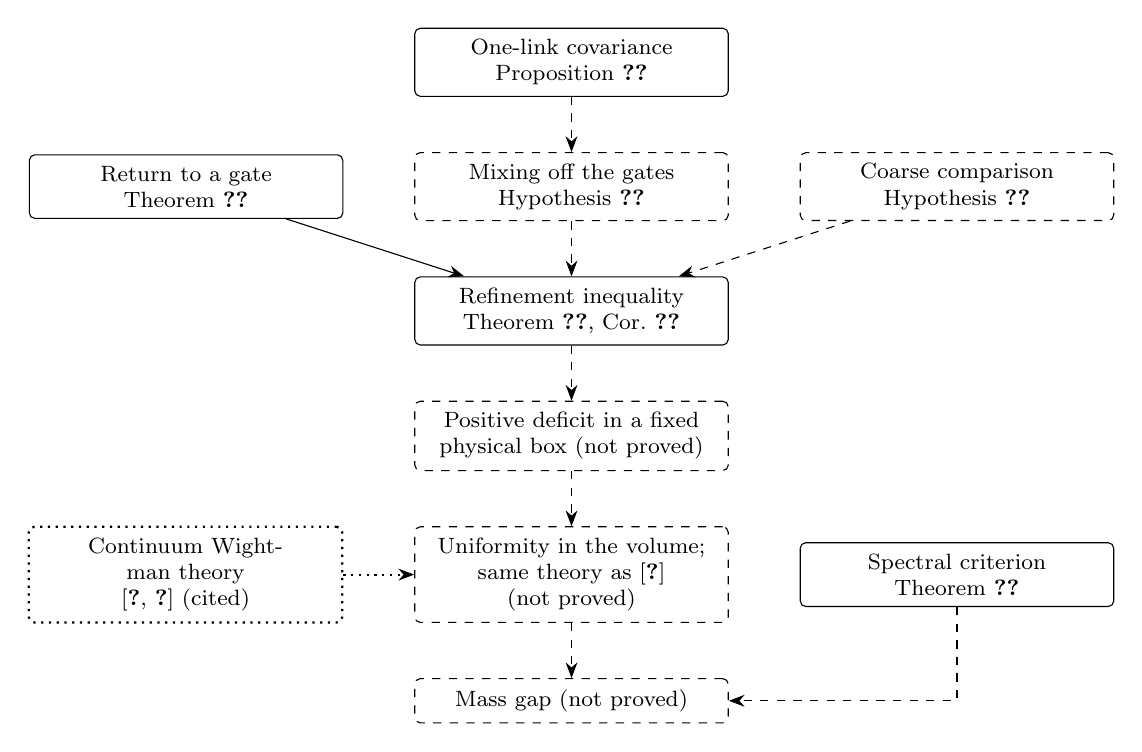
\begin{tikzpicture}[node distance=7mm and 9mm,
 prov/.style={draw,rounded corners=2pt,align=center,font=\footnotesize,inner sep=4pt,text width=37mm},
 open/.style={prov,dashed},
 ext/.style={prov,dotted,thick},
 >={Stealth[length=2mm]}]
\node[prov] (ret) {Return to a gate\\ Theorem~\ref{t:ret}};
\node[open,right=of ret] (mix) {Mixing off the gates\\ Hypothesis~\ref{h:mix}};
\node[open,right=of mix] (coarse) {Coarse comparison\\ Hypothesis~\ref{h:coarse}};
\node[prov,below=of mix] (inh) {Refinement inequality\\ Theorem~\ref{t:inh}, Cor.~\ref{c:acc}};
\node[open,below=of inh] (box) {Positive deficit in a fixed\\ physical box (not proved)};
\node[open,below=of box] (vol) {Uniformity in the volume;\\ same theory as~\cite{OAI} (not proved)};
\node[ext,left=of vol] (ext) {Continuum Wightman theory\\ \cite{OAI,YMG} (cited)};
\node[prov,right=of vol] (crit) {Spectral criterion\\ Theorem~\ref{t:crit}};
\node[open,below=of vol] (gap) {Mass gap (not proved)};
\node[prov,above=of mix] (haar) {One-link covariance\\ Proposition~\ref{p:haar}};
\draw[->] (ret) -- (inh);
\draw[->,dashed] (mix) -- (inh);
\draw[->,dashed] (coarse) -- (inh);
\draw[->,dashed] (inh) -- (box);
\draw[->,dashed] (box) -- (vol);
\draw[->,dashed] (vol) -- (gap);
\draw[->,dotted,thick] (ext) -- (vol);
\draw[->,dashed] (crit) |- (gap);
\draw[->,dashed] (haar) -- (mix);
\end{tikzpicture}
\caption{Dependencies. Solid: proved here. Dashed: open; dashed arrows are implications that would hold if the
open statements at their tails were proved, with the inputs named in the text. Dotted: cited, not verified
here. Proposition~\ref{p:haar} supplies a lower bound for one term that enters Hypothesis~\ref{h:mix}; it does
not prove it.}\label{f:arch}
\end{figure}

\begin{hypothesis}[Mixing off the gates; open]\label{h:mix}
For a sequence of lattices of mesh $a_i\to0$ in a fixed physical box, with exceptional projections $B_i$ built
from gates as in Theorem~\ref{t:ret}, there are $\gamma_i>0$ with $\langle f,(I-S_{2a_i})f\rangle\ge
\gamma_i\|G_if\|^2$ for all centred $f$, and $\sum_ia_i/\gamma_i<\infty$.
\end{hypothesis}

\begin{hypothesis}[Coarse comparison; open]\label{h:coarse}
With $d_{i-1}$ the deficit of the lattice of mesh $2a_i$ at the same physical time $t$ and matched coupling,
$\|P_iS^{(i)}_tP_i\|\le1-b_i$ with $b_i\ge d_{i-1}-\varepsilon_i$ and $\sum_i\varepsilon_i$ small against
$d_0$.
\end{hypothesis}

Neither hypothesis is known for any interacting lattice gauge theory in four dimensions. Section~\ref{s:evid}
reports what was measured about each. If both held, together with Theorem~\ref{t:ret} and a summable choice
of gates, Corollary~\ref{c:acc} would give a positive lower limit of the deficits in a fixed physical box. That
is still not a mass gap: uniformity in the volume and the identification of the limit with a continuum theory
would remain, and Theorem~\ref{t:crit} is the form in which a gap would then have to be verified on a total
family of vectors.

\section{The spectral criterion}\label{s:crit}
\begin{proof}[Proof of Theorem~\ref{t:crit}]
Let $E$ be the spectral measure of $H$ and $\mu_v(\cdot)=\langle v,E(\cdot)v\rangle$, a finite positive measure
on $[0,\infty)$. Then $d_{v,n}=\int_{[0,\infty)}e^{-n\tau s}(1-e^{-\tau s})\,d\mu_v(s)$; the integrand is
non-negative and vanishes at $s=0$.

(1)$\Rightarrow$(2). If $\mu_v$ gives no mass to $(0,\Delta)$ then $d_{v,n}\le e^{-n\tau\Delta}\|v\|^2=r^n\|v\|^2$.

(2)$\Rightarrow$(1). Let $v\in D$ and suppose $\mu_v((0,\Delta))>0$. Then there are $0<\alpha<\omega<\Delta$ with
$\mu_v([\alpha,\omega])>0$, and $d_{v,n}\ge e^{-n\tau\omega}(1-e^{-\tau\alpha})\mu_v([\alpha,\omega])$, so
$\limsup d_{v,n}^{1/n}\ge e^{-\tau\omega}>r$, a contradiction. Hence $E((0,\Delta))v=0$ for every $v\in D$.
The projection $E((0,\Delta))$ is bounded and vanishes on a set with dense span, so it is zero.
\end{proof}

\begin{remark}\label{r:crit}
(a) Positivity is what prevents cancellation: the criterion is stated on the diagonal, for single vectors. A
bound on a matrix element $\langle v,e^{-n\tau H}w\rangle$ follows from it by polarisation and gives nothing
more. (b) A polynomial bound on the low-energy weight, $\mu_v((0,s])\le Cs^p$, does not give (2) for any
$r<1$. (c) In a theory with several vacua or several pure phases, the criterion may be applied in one
component; a gap there says nothing about the others.
\end{remark}

\section{The refinement inequality}\label{s:inh}
\begin{lemma}\label{l:scal}
For $0\le x\le1$ and real $\rho\ge0$, $x(1-x^\rho)\le\rho(1-x)$.
\end{lemma}
\begin{proof}
For $x=0$ both sides are non-negative and the left is $0$. For $0<x\le1$, $1-x^\rho\le-\rho\log x$ because
$1-e^{-s}\le s$, and $-x\log x\le1-x$ because $\log(1/x)\le1/x-1$.
\end{proof}

\begin{proof}[Proof of Theorem~\ref{t:inh}]
Fix $L>\lambda$ and let $E=\mathbf 1_{[0,L]}(H)$, which is not zero. Since $E$ commutes with $H$ and
$S_s(I-E)\ge0$, we have $S_s\ge S_sE\ge e^{-sL}E$ for every $s\ge0$. Let $v$ be a unit vector in the range of
$E$.

\emph{Good part.} By the first hypothesis, $\gamma\|Gv\|^2\le\langle v,(I-S_{2a})v\rangle\le1-e^{-2aL}$.

\emph{Exceptional part.} $BS_\tau B\ge e^{-\tau L}BEB$, so $\|EB\|^2=\|BEB\|\le e^{\tau L}\kappa$, and
$\|Bv\|=\|BEv\|\le\|BE\|=\|EB\|$. Hence $\|Bv\|^2\le e^{\tau L}\kappa$.

\emph{Coarse part.} In the same way $\|Pv\|^2\le\|EP\|^2=\|PEP\|\le e^{tL}\|PS_tP\|\le e^{tL}(1-b)$.

Since $B$ and $G$ are orthogonal projections with $B+G=Q$ and $BG=0$, $\|Qv\|^2=\|Gv\|^2+\|Bv\|^2$, and
$\|Pv\|^2=1-\|Qv\|^2$. Therefore
\[
1-e^{tL}(1-b)\ \le\ \frac{1-e^{-2aL}}{\gamma}+e^{\tau L}\kappa .
\]
Multiply by $x=e^{-tL}\in(0,1]$ and use $e^{-(t-\tau)L}\le1$: with $\rho=2a/t$,
\[
b\ \le\ 1-x+\frac{x(1-x^{\rho})}{\gamma}+\kappa\ \le\ (1-x)\Big(1+\frac{\rho}{\gamma}\Big)+\kappa
\]
by Lemma~\ref{l:scal}. Let $L\downarrow\lambda$: $1-e^{-t\lambda}\ge(b-\kappa)/(1+\rho/\gamma)$. As
$1-e^{-t\lambda}\ge0$, \eqref{e:inh} follows.
\end{proof}

\begin{corollary}[Accumulation]\label{c:acc}
Let $d_0\ge0$ and, for $i=1,\dots,n$, let $K_i>0$, $\kappa_i,\varepsilon_i,b_i,d_i\in\R$ satisfy
$d_i\ge(b_i-\kappa_i)/K_i$ and $b_i\ge d_{i-1}-\varepsilon_i$. With $M_0=1$ and $M_i=K_1\cdots K_i$,
\[
d_n\ \ge\ M_n^{-1}\Big(d_0-\sum_{i=1}^nM_{i-1}(\varepsilon_i+\kappa_i)\Big).
\]
With $K_i=1+2a_i/(\gamma_it)$, the product $M_n$ stays bounded if and only if $\sum_ia_i/\gamma_i<\infty$.
\end{corollary}
\begin{proof}
$M_id_i\ge M_{i-1}(b_i-\kappa_i)\ge M_{i-1}d_{i-1}-M_{i-1}(\varepsilon_i+\kappa_i)$; sum over $i$.
\end{proof}

\begin{remark}[Rarity alone is not enough]\label{r:reset}
The second hypothesis in~\eqref{e:hyp} is about return at a later time, not about the probability of the
exceptional set. For the reversible process $S_t=e^{-\ell t}I+(1-e^{-\ell t})\E$ and an exceptional event of
arbitrarily small probability carrying two equally likely fine labels, the difference of the labels gives
$\|BS_tB\|=e^{-\ell t}$ whatever the probability of the event.
\end{remark}

\section{Return to a coarse plaquette gate}\label{s:ret}
\begin{lemma}[Caps under a tilted law]\label{l:cap}
Let $u\in S^3$ have density $f_k(u)=e^{k\,u\cdot v}/Z(k)$ with respect to the uniform probability measure,
$k\ge0$, $v$ a unit vector. For every $c\in S^3$ and $0\le\theta\le\pi$, the probability of the cap
$\{u:\operatorname{dist}(u,c)\le\theta\}$ is at most that of the cap of the same radius centred at $v$, which
equals $p_k(\theta)$ and is non-decreasing in $k$.
\end{lemma}
\begin{proof}
The superlevel sets $\{f_k>s\}$ are caps centred at $v$. For a cap $C'$ centred at $c$ and the cap $C$ of the
same radius centred at $v$, the uniform measure of $\{f_k>s\}\cap C'$ is at most the smaller of the measures of
the two sets, which is the measure of $\{f_k>s\}\cap C$ because those two caps are concentric. Integrating
over $s$ gives $\int_{C'}f_k\le\int_Cf_k$. In the polar angle $r$ from $v$ the uniform measure is
$\tfrac2\pi\sin^2r\,dr$, which gives the formula for $p_k$. Finally $\frac{d}{dk}\P_k(C)=
\Cov_k(\mathbf 1_{\{r\le\theta\}},\cos r)\ge0$, because both are non-increasing functions of $r$.
\end{proof}

\begin{proof}[Proof of Theorem~\ref{t:ret}]
Let $y$ be the later slice and let $U$ be one of the eight fine links of the coarse plaquette in that slice.
Condition on all other links of the lattice; these include every link of the slice $x$, because the two
slices are distinct. The holonomy is $XUY$ with $X,Y$ fixed, and $\operatorname{dist}(XUY,-I)=
\operatorname{dist}(U,-X^{-1}Y^{-1})$ by invariance of the round distance, so the event $y\in A_\theta$ is a cap of
radius $\theta$ for $U$. The conditional density of $U$ is proportional to $\exp(\beta\,\tfrac12\Tr(U\Sigma))$
with $\Sigma$ the sum of the six staples of the link, each a unit quaternion; writing $\Sigma=|\Sigma|\,v^{-1}$
this is $e^{k\,u\cdot v}$ with $k=\beta|\Sigma|\le6\beta$. By Lemma~\ref{l:cap},
$\P(y\in A_\theta\mid\text{all other links})\le p_{6\beta}(\theta)$, and by the tower property
$\P(y\in A_\theta\mid x)\le p_{6\beta}(\theta)$ almost surely.

The joint law of $(x,y)$ is invariant under exchanging the two slices (reflection of the periodic time
direction about the midpoint between them, composed with a translation). With $h=\mathbf 1_{A_\theta}g$,
\[
|\E[h(x)h(y)]|\le\tfrac12\E\big[\mathbf 1_{A_\theta}(x)\mathbf 1_{A_\theta}(y)(g(x)^2+g(y)^2)\big]
=\E\big[\mathbf 1_{A_\theta}(x)g(x)^2\,\P(y\in A_\theta\mid x)\big],
\]
which is at most $p_{6\beta}(\theta)\E[\mathbf 1_{A_\theta}(x)g(x)^2]$.

For the envelope: the numerator of $p_k$ is at most $\theta^3/3$. On $0\le r\le(1+k)^{-1/2}\le1$ we have
$\sin r\ge2r/\pi$ and $k(1-\cos r)\le kr^2/2\le\tfrac12$, so the denominator is at least
$\tfrac{4}{\pi^2}e^{-1/2}\cdot\tfrac13(1+k)^{-3/2}$.
\end{proof}

\begin{remark}\label{r:ret}
(a) For a union of $M$ gates of radius $\theta$ the same proof gives the bound
$\min(1,Mp_{6\beta}(\theta))$; no independence between plaquettes is used. Take all the
$M=3(N/2)^3$ coarse plaquettes and the radius $\theta=c(1+6\beta)^{-1/2}N^{-4/3}$. Then the bound is at most
\[\tfrac{3\pi^2\sqrt e}{32}\,c^3/N,\]
which is summable over dyadic $N$. (b) At $\beta=3.399810242$ the bound $p_{6\beta}(\theta)$ is $0.00307$, $0.156$ and $0.935$ for
$\theta=0.05$, $0.2$ and $0.6$. The gates it controls are narrow; Section~\ref{s:evid} shows that the region of
slow local relaxation around $-I$ is not. (c) In terms of Theorem~\ref{t:inh}: with $R$ multiplication by the
indicator of a union of gates, which is coarse-measurable and so commutes with $P$, the projection $B=RQ$ has
range inside that of $R$, and~\eqref{e:ret} bounds $\|BS_\tau B\|$ for the two-slice operator of the periodic
lattice at any lag of at least one time step.
\end{remark}

\section{The one-link covariance}\label{s:haar}
\begin{proof}[Proof of Proposition~\ref{p:haar}]
With $Z(k)=\int e^{k\,u\cdot v}du=2I_1(k)/k$, the mean of $u\cdot v$ is $(\log Z)'=I_1'/I_1-1/k=I_2/I_1=R$ by
$I_1'=I_2+I_1/k$, and its variance is $R'$. By symmetry the covariance is a multiple of the identity on
$v^\perp$; since $|u|=1$, its trace there is $1-\E(u\cdot v)^2=1-R'-R^2$. From $I_1'=I_2+I_1/k$ and
$I_2'=I_1-2I_2/k$~\cite[10.29.2]{DLMF},
\begin{equation}\label{e:ric}
p:=R'=1-\frac{3R}{k}-R^2,
\end{equation}
so the transverse eigenvalue is $(3R/k)/3=q:=R/k$. Differentiating,
\[
p'=-\Big(2R+\frac3k\Big)p+\frac{3R}{k^2},\qquad q'=\frac{p-q}{k},\qquad
w'=3R-\Big(2R+\frac1k\Big)w\ \text{ for }w:=k^2p .
\]
From the series $R=k/4-k^3/96+O(k^5)$: $p-q=-k^2/48+O(k^4)$, $p'=-k/16+O(k^3)$ and $w'=k/2+O(k^3)$ as
$k\downarrow0$. Each of the three claims is that a continuously differentiable function $\phi$ on $(0,\infty)$,
of a definite sign near $0$, has no zero; if it had one, the zero set, closed in $(0,\infty)$, would have a
least element $k_0$, and $\phi'(k_0)$ would have the sign opposite to that of $\phi$ near $0$, or vanish.

\emph{$p<q$.} Take $\phi=p-q<0$ near $0$. At a zero, $q'=0$ and $p'=-(2R+3/k)q+3q/k=-2Rq<0$, so $\phi'<0$:
impossible at a first zero of a function negative before it.

\emph{$p'<0$.} Take $\phi=p'<0$ near $0$. Differentiating the equation for $p'$ and setting $p'=0$ gives
$p''=-2p^2+6(p-q)/k^2<0$ by the previous step: impossible.

\emph{$w'>0$.} Take $\phi=w'>0$ near $0$. At a zero of $w'$, $w=3R/(2R+1/k)<\tfrac32$ and
$w''=3p-(2p-1/k^2)w=p(4-2w)>0$, using $w/k^2=p$ and $p>0$: impossible.

For the last statement, if $\beta\ge1$ and $0<k\le L\beta$ then
$\beta^2m(k)=\beta^2p(k)\ge\beta^2p(L\beta)=w(L\beta)/L^2\ge w(L)/L^2=p(L)$. The enclosure of $R'(6)$ follows
from~\eqref{e:ric} and the power series of $I_1,I_2$ summed in rational arithmetic with a geometric bound on
the tail (33 terms).
\end{proof}

\begin{remark}\label{r:haar}
The conditional law of one link given the others is of this form with $k\le6\beta$ (as in the proof of
Theorem~\ref{t:ret}), so every unit linear functional of one link has conditional variance at least
$R'(6)/\beta^2$ for $\beta\ge1$. This is a lower bound for losses of the kind that enter
Hypothesis~\ref{h:mix}. It is a bound on a loss, not on the quotient of loss by variance, and it is three to
four orders of magnitude below the losses measured in Section~\ref{s:evid}.
\end{remark}

\section{Measurements bearing on the two hypotheses}\label{s:evid}
All numbers in this section are Monte Carlo estimates for $\SU(2)$ with jackknife errors over independent
streams; programs, seeds, raw data or the commands that regenerate them, the predicates fixed before each run
and those that failed are in~\cite{Repo}. They are stated to show what the open hypotheses face, not to
support them.

\subsection{The local quotient on a frozen coarse background}\label{s:local}
Side $N=6$, $T=12$, $\beta=3.276133577$ (a point of a line of constant renormalised coupling determined
in~\cite{Repo}; we did not recalibrate it). The coarse links of one slice are frozen: all equal to the
identity except two, chosen so that one coarse plaquette has holonomy $-I$ and a neighbouring one supplies a
reference direction. The tests are linear combinations of gauge-invariant marks built from the fine
plaquettes inside coarse plaquettes. The combination with the smallest quotient $\mathcal J/\mathcal V$ is
found on $16$ streams and its quotient is evaluated on $16$ others (Table~\ref{tab:local}).

\begin{table}[ht]
\centering\small
\begin{tabular}{@{}p{0.36\textwidth}cccc@{}}
\toprule
Number of marks & 15 & 49 & 181 & 308 \\
\midrule
background with a $-I$ plaquette & .0208(5) & .0167(4) & .0159(4) & .0154(4) \\
background sampled from the measure, every coarse plaquette at distance $>1.1$ from $-I$ & .0589(8) & .0533(5) & .0510(4) & .0428(4) \\
\bottomrule
\end{tabular}
\caption{Smallest local quotient $\mathcal J/\mathcal V$ found in a span of marks, evaluated on held-out
streams. For comparison, the single mark used first gives $.047$ and $.09$ on the two backgrounds.}
\label{tab:local}
\end{table}

Three observations. (i) The optimum is a collective combination: $81$ per cent of its weight lies on the three
coarse plaquettes through the frozen link that was changed, with opposite signs on neighbouring plaquettes.
(ii) On the background with a $-I$ plaquette the optimum decreases more and more slowly as the span grows; on
the sampled background it is still decreasing at the largest span. In neither case is a lower bound for the
quotient over all tests indicated; these are upper bounds for it. (iii) Displacing the frozen holonomy from
$-I$ by round distances up to $2/\beta$ leaves the quotient of the first single mark unchanged within the
errors (ratio $1.004(11)$ at $2/\beta$ in a repeated run), so the low quotient is not confined to the narrow
gates that Theorem~\ref{t:ret} controls.

\subsection{Persistence in time of the slow local combination}\label{s:time}
In the same ensemble (one slice frozen, all else free) the optimal $308$-mark combination of the frozen slice
was regressed on the same marks one time slice later, in two gauge-invariant forms. By a rule fixed before the
runs, persistence would have been declared if the held-out coefficient of determination exceeded $0.1$. It is
$-0.013(2)$ and $-0.002(2)$ in the two forms; with $308$ regressors the estimator has a negative bias of about
$0.017$, and a regression on $15$ marks gives $0.011(2)$. A correlation of $0.083(6)$ at one step, against
$0.032(5)$ on a sampled background, is resolved; at two steps nothing is. So a combination whose local loss is
$1.5$ per cent of its variance is carried to the next time slice with a coefficient of determination of about
one per cent. On this evidence, slow relaxation under the local resampling near $-I$ is not slow propagation in
time. This is one background, one size and one coupling, and the combination tested is the slowest for the
local resampling, which need not be the slowest in time.

\subsection{Comparison across a factor of two in the mesh}\label{s:cross}
Sides $N=5$ and $N=10$ at couplings $3.196581051$ and $3.493705679$ (matched in~\cite{Repo} at a fixed
renormalised coupling; not recalibrated here), time extents two and four times the side, and the same physical
lag (one and two time steps). The tests are $54$ functions of the coarse links of side $10$, respectively of
the links of side $5$, defined by the same formulas. For a test $f$ let
$\mathsf R(f)=1-C_f(\mathrm{lag})/C_f(0)$ with $C_f$ its connected two-time correlation.
\begin{enumerate}
\item An unnormalised comparison of two-time energies, $\mathcal E_{10}(f)\ge c\,\mathcal E_5(f)$, fails for a
frozen test unless $c\le0.005$: the stationary variance of the same function of coarse links is $0.0034$ times
smaller on the finer lattice. Any comparison of the kind in Hypothesis~\ref{h:coarse} must be normalised by
the variance.
\item In the normalised form, one test chosen on training streams and then frozen has
$\mathsf R_{10}(f)/\mathsf R_5(f)=0.941(5)$ on held-out streams and $0.936(3)$ on independent ensembles of the
longer time extent: this function of coarse links keeps more correlation on the finer lattice. A constant
$\alpha>0.95$ in $\mathsf R_{10}\ge\alpha\mathsf R_5$ is therefore excluded for this pair by a single test. This
does not decide Hypothesis~\ref{h:coarse}, which compares the worst cases on the two lattices and not one
test; it shows that the comparison is not an identity and that a loss $\varepsilon_i$ of several per cent of
$\mathsf R$ per halving of the mesh has to be expected at this scale.
\item A span of $16$ functions had shown no such test. The result depends on the span.
\end{enumerate}

\section{Machine-checked parts}\label{s:lean}
Two Lean~4 files with Mathlib accompany the paper in~\cite{Repo}; both compile with no \texttt{sorry} and use
only the axioms \texttt{propext}, \texttt{Classical.choice} and \texttt{Quot.sound}.
\begin{itemize}
\item \texttt{Inheritance.lean}: Lemma~\ref{l:scal} for real exponents; the scalar conclusion of
Theorem~\ref{t:inh}; Corollary~\ref{c:acc}; and Theorem~\ref{t:inh} for a real finite-dimensional space, with
$H$ given by an orthonormal eigenbasis and non-negative eigenvalues. The three inequalities~\eqref{e:hyp}
are hypotheses of the formal statement. The infinite-dimensional case, proved above, is not formalised.
\item \texttt{haar.lean}: the algebra at the zeros in the proof of Proposition~\ref{p:haar}, given the three
differential relations as hypotheses, the reduction $\beta^2m(k)\ge R'(L)$ given the monotonicities, and the
first-zero principle. The Bessel identities themselves are not formalised.
\end{itemize}
Theorems~\ref{t:crit} and~\ref{t:ret} are not formalised.

\section{What remains}\label{s:rem}
Table~\ref{tab:status} lists every statement and its status. To turn the architecture of
Figure~\ref{f:arch} into a proof of a mass gap one would need, at least: Hypothesis~\ref{h:mix} with gates wide
enough to contain the region of slow local relaxation and still summable under a bound of the kind of
Theorem~\ref{t:ret}; Hypothesis~\ref{h:coarse} with summable losses; the passage of Theorem~\ref{t:ret} to the
vacuum on an infinite time axis; estimates uniform in the physical volume; the identification of the limiting
semigroup with the Hamiltonian of a continuum theory satisfying the axioms, for which~\cite{OAI} is a
candidate that we have not connected to these lattices; and all of this for every compact simple group, where
the argument of Section~\ref{s:ret} has no analogue for groups with trivial centre. We cannot estimate the
distance to any of these.

\begin{table}[ht]
\centering\small
\begin{tabular}{@{}p{0.34\textwidth}p{0.6\textwidth}@{}}
\toprule
Statement & Status \\
\midrule
Theorem~\ref{t:crit} & proved (Section~\ref{s:crit}) \\
Theorem~\ref{t:inh}, Corollary~\ref{c:acc} & proved; finite-dimensional case and scalar steps checked in Lean \\
Theorem~\ref{t:ret} & proved for periodic time; $\SU(2)$ only \\
Proposition~\ref{p:haar} & proved; scalar steps checked in Lean \\
Hypothesis~\ref{h:mix} & open; Table~\ref{tab:local} gives upper bounds for the best possible rate on two backgrounds \\
Hypothesis~\ref{h:coarse} & open; one pair of lattices measured (Section~\ref{s:cross}) \\
Volume uniformity; continuum identification & open; not addressed \\
Mass gap & not proved \\
\bottomrule
\end{tabular}
\caption{Status of every statement.}\label{tab:status}
\end{table}

Results on reduced models obtained in the same project, among them an upper bound on the lattice gap at weak
coupling and the weak-coupling spectrum of the theory on a single spatial site, are in separate
manuscripts in~\cite{Repo} and are not used here.

\begin{thebibliography}{9}
\bibitem{DLMF} \emph{NIST Digital Library of Mathematical Functions}, \S10.29, \url{https://dlmf.nist.gov/10.29}.
\bibitem{JW} A.~Jaffe and E.~Witten, \emph{Quantum Yang--Mills theory}, Clay Mathematics Institute problem
description, \url{https://www.claymath.org/wp-content/uploads/2022/06/yangmills.pdf}. Sections 4 and 5 read.
\bibitem{OAI} OpenAI, Lean formalisation of a construction of continuum Yang--Mills theory, submitted
28 October 2026, repository \texttt{yang-mills-group/OpenAI-YM-20261028}. Not read by us; cited through~\cite{YMG}.
\bibitem{Repo} K.~Justus, research repository \texttt{KirtusJ/Millennium-Prize-Problems}, folders
\texttt{yang-mills/z4/attempt/reviews} (measurements, Lean files, review records) and
\texttt{yang-mills/joint-refinement} (the derivations by sessions of OpenAI Codex on which
Theorems~\ref{t:inh} and~\ref{t:ret} are based).
\bibitem{YMG} Yang--Mills group, \emph{Validation of the OpenAI Yang--Mills construction}, release of
10 November 2026, \url{https://alexisdpc.github.io/yang-mills/references/assessment-1-2026-11-10.pdf}. First page
and Part~I contents read; the statement quoted is on p.~1.
\end{thebibliography}
\end{document}
